% Options for packages loaded elsewhere
\PassOptionsToPackage{unicode}{hyperref}
\PassOptionsToPackage{hyphens}{url}
%
\documentclass[
]{article}
\usepackage{lmodern}
\usepackage{amssymb,amsmath}
\usepackage{ifxetex,ifluatex}
\ifnum 0\ifxetex 1\fi\ifluatex 1\fi=0 % if pdftex
  \usepackage[T1]{fontenc}
  \usepackage[utf8]{inputenc}
  \usepackage{textcomp} % provide euro and other symbols
\else % if luatex or xetex
  \usepackage{unicode-math}
  \defaultfontfeatures{Scale=MatchLowercase}
  \defaultfontfeatures[\rmfamily]{Ligatures=TeX,Scale=1}
\fi
% Use upquote if available, for straight quotes in verbatim environments
\IfFileExists{upquote.sty}{\usepackage{upquote}}{}
\IfFileExists{microtype.sty}{% use microtype if available
  \usepackage[]{microtype}
  \UseMicrotypeSet[protrusion]{basicmath} % disable protrusion for tt fonts
}{}
\makeatletter
\@ifundefined{KOMAClassName}{% if non-KOMA class
  \IfFileExists{parskip.sty}{%
    \usepackage{parskip}
  }{% else
    \setlength{\parindent}{0pt}
    \setlength{\parskip}{6pt plus 2pt minus 1pt}}
}{% if KOMA class
  \KOMAoptions{parskip=half}}
\makeatother
\usepackage{xcolor}
\IfFileExists{xurl.sty}{\usepackage{xurl}}{} % add URL line breaks if available
\IfFileExists{bookmark.sty}{\usepackage{bookmark}}{\usepackage{hyperref}}
\hypersetup{
  hidelinks,
  pdfcreator={LaTeX via pandoc}}
\urlstyle{same} % disable monospaced font for URLs
\usepackage[margin=1in]{geometry}
\usepackage{color}
\usepackage{fancyvrb}
\newcommand{\VerbBar}{|}
\newcommand{\VERB}{\Verb[commandchars=\\\{\}]}
\DefineVerbatimEnvironment{Highlighting}{Verbatim}{commandchars=\\\{\}}
% Add ',fontsize=\small' for more characters per line
\usepackage{framed}
\definecolor{shadecolor}{RGB}{248,248,248}
\newenvironment{Shaded}{\begin{snugshade}}{\end{snugshade}}
\newcommand{\AlertTok}[1]{\textcolor[rgb]{0.94,0.16,0.16}{#1}}
\newcommand{\AnnotationTok}[1]{\textcolor[rgb]{0.56,0.35,0.01}{\textbf{\textit{#1}}}}
\newcommand{\AttributeTok}[1]{\textcolor[rgb]{0.77,0.63,0.00}{#1}}
\newcommand{\BaseNTok}[1]{\textcolor[rgb]{0.00,0.00,0.81}{#1}}
\newcommand{\BuiltInTok}[1]{#1}
\newcommand{\CharTok}[1]{\textcolor[rgb]{0.31,0.60,0.02}{#1}}
\newcommand{\CommentTok}[1]{\textcolor[rgb]{0.56,0.35,0.01}{\textit{#1}}}
\newcommand{\CommentVarTok}[1]{\textcolor[rgb]{0.56,0.35,0.01}{\textbf{\textit{#1}}}}
\newcommand{\ConstantTok}[1]{\textcolor[rgb]{0.00,0.00,0.00}{#1}}
\newcommand{\ControlFlowTok}[1]{\textcolor[rgb]{0.13,0.29,0.53}{\textbf{#1}}}
\newcommand{\DataTypeTok}[1]{\textcolor[rgb]{0.13,0.29,0.53}{#1}}
\newcommand{\DecValTok}[1]{\textcolor[rgb]{0.00,0.00,0.81}{#1}}
\newcommand{\DocumentationTok}[1]{\textcolor[rgb]{0.56,0.35,0.01}{\textbf{\textit{#1}}}}
\newcommand{\ErrorTok}[1]{\textcolor[rgb]{0.64,0.00,0.00}{\textbf{#1}}}
\newcommand{\ExtensionTok}[1]{#1}
\newcommand{\FloatTok}[1]{\textcolor[rgb]{0.00,0.00,0.81}{#1}}
\newcommand{\FunctionTok}[1]{\textcolor[rgb]{0.00,0.00,0.00}{#1}}
\newcommand{\ImportTok}[1]{#1}
\newcommand{\InformationTok}[1]{\textcolor[rgb]{0.56,0.35,0.01}{\textbf{\textit{#1}}}}
\newcommand{\KeywordTok}[1]{\textcolor[rgb]{0.13,0.29,0.53}{\textbf{#1}}}
\newcommand{\NormalTok}[1]{#1}
\newcommand{\OperatorTok}[1]{\textcolor[rgb]{0.81,0.36,0.00}{\textbf{#1}}}
\newcommand{\OtherTok}[1]{\textcolor[rgb]{0.56,0.35,0.01}{#1}}
\newcommand{\PreprocessorTok}[1]{\textcolor[rgb]{0.56,0.35,0.01}{\textit{#1}}}
\newcommand{\RegionMarkerTok}[1]{#1}
\newcommand{\SpecialCharTok}[1]{\textcolor[rgb]{0.00,0.00,0.00}{#1}}
\newcommand{\SpecialStringTok}[1]{\textcolor[rgb]{0.31,0.60,0.02}{#1}}
\newcommand{\StringTok}[1]{\textcolor[rgb]{0.31,0.60,0.02}{#1}}
\newcommand{\VariableTok}[1]{\textcolor[rgb]{0.00,0.00,0.00}{#1}}
\newcommand{\VerbatimStringTok}[1]{\textcolor[rgb]{0.31,0.60,0.02}{#1}}
\newcommand{\WarningTok}[1]{\textcolor[rgb]{0.56,0.35,0.01}{\textbf{\textit{#1}}}}
\usepackage{longtable,booktabs}
% Correct order of tables after \paragraph or \subparagraph
\usepackage{etoolbox}
\makeatletter
\patchcmd\longtable{\par}{\if@noskipsec\mbox{}\fi\par}{}{}
\makeatother
% Allow footnotes in longtable head/foot
\IfFileExists{footnotehyper.sty}{\usepackage{footnotehyper}}{\usepackage{footnote}}
\makesavenoteenv{longtable}
\usepackage{graphicx,grffile}
\makeatletter
\def\maxwidth{\ifdim\Gin@nat@width>\linewidth\linewidth\else\Gin@nat@width\fi}
\def\maxheight{\ifdim\Gin@nat@height>\textheight\textheight\else\Gin@nat@height\fi}
\makeatother
% Scale images if necessary, so that they will not overflow the page
% margins by default, and it is still possible to overwrite the defaults
% using explicit options in \includegraphics[width, height, ...]{}
\setkeys{Gin}{width=\maxwidth,height=\maxheight,keepaspectratio}
% Set default figure placement to htbp
\makeatletter
\def\fps@figure{htbp}
\makeatother
\setlength{\emergencystretch}{3em} % prevent overfull lines
\providecommand{\tightlist}{%
  \setlength{\itemsep}{0pt}\setlength{\parskip}{0pt}}
\setcounter{secnumdepth}{-\maxdimen} % remove section numbering

\author{}
\date{\vspace{-2.5em}}

\begin{document}

\hypertarget{seasonal-adjustment-of-daily-time-series-in-r-an-overview}{%
\section{Seasonal adjustment of daily time series in R: An
overview}\label{seasonal-adjustment-of-daily-time-series-in-r-an-overview}}

Automated data processing and the Internet have brought an enormous
increase in data that is processed on a high frequency, e.g., at a
daily, hourly or even higher frequency. While some higher frequency
series have been used in the past (e.g., Fisher 1923, cited by Ladiray
2018) these series are much more abundant now. X-13ARIMA-SEATS offers a
well tested and time proven way of adjusting monthly, quarterly (or
bi-annual) series, but it cannot deal with data at a higher frequency.

This {[}article/chaper/post{]} discusses how to perform seasonal
adjustment on a higher frequency. We focus on daily data, as this is the
most common use case, but will briefly discuss some challenges involving
weekly or intra-day adjustments.

Despite the large interest, there is not much consensus on the
appropriate adjustment method for daily series. Adjusting daily series
often involves a substantial amount of trial and error, subjective
judgment and exploration. This {[}article/chapter/post{]} gives an
overview of the tools that are currently (2021) available in R.

\hypertarget{contribution-of-this-articlechaperpost}{%
\subsection{Contribution of this
{[}article/chaper/post{]}}\label{contribution-of-this-articlechaperpost}}

\begin{itemize}
\tightlist
\item
  Discuss literature on daily seasonal adjustment
\item
  Overview of available methods in R (including examples)
\item
  OOS forecast evaluation of available methods in R
\item
  Discuss specific problems
\end{itemize}

\hypertarget{problems}{%
\subsection{Problems}\label{problems}}

Daily seasonal adjustment comes with a few challenges that are not
present in lower frequency data. Let's focus on daily traffic
casualties.

First, daily data comes at multiple periodicities: There is an annual
periodicity, such as the effect of weather condiditions or holiday
patterns. Then there is a weekly periodicity. Casualities may be higher
during the weekdays, due to increased work traffic. For some series,
there may be also a monthly periodicity. If people are get their
salaries by the end of the month, they may be more likely to perform
certain investments.

Second, many daily data series are available for a few years only.
Whily, e.g., the SEATS adjustment requires a minimal series length of XX
years, many daily series are shorter.

Third, higher frequency series are generally more volatile and prone to
outliers.

Fourth, the effect of individual holiday is challenging to estimate.
Often, economic effects of holidays may occur before or after a holiday,
thus lagging or leading them is crucial.

\hypertarget{parametric-versus-non-parametric-models}{%
\subsection{Parametric versus Non-parametric
Models}\label{parametric-versus-non-parametric-models}}

Various attempts to seasonly adjust data can be broadly distinguished
into parametric and non-parametric approaches. Non-parametric approaches
seem to be the more obvious candidates to use with the irregular
structure of daily data. Parametric models require the time units to be
regularly spaced. Non-parametric estimation is also what is used in the
X-11 method of X-13.

\hypertarget{r-packages}{%
\subsection{R Packages}\label{r-packages}}

As mentioned before, there is no accepted consensus on how to perform
daily seasonal adjustment. In the following, we discuss various
possibilities to adjust series in R. We focus on a single time series,
and describe the concrete steps that are required to perform an
adjustment.

\begin{Shaded}
\begin{Highlighting}[]
\KeywordTok{library}\NormalTok{(dailyadj)}
\KeywordTok{library}\NormalTok{(tsbox)}

\NormalTok{x <-}\StringTok{ }\NormalTok{casualties}

\KeywordTok{ts_plot}\NormalTok{(x)}
\end{Highlighting}
\end{Shaded}

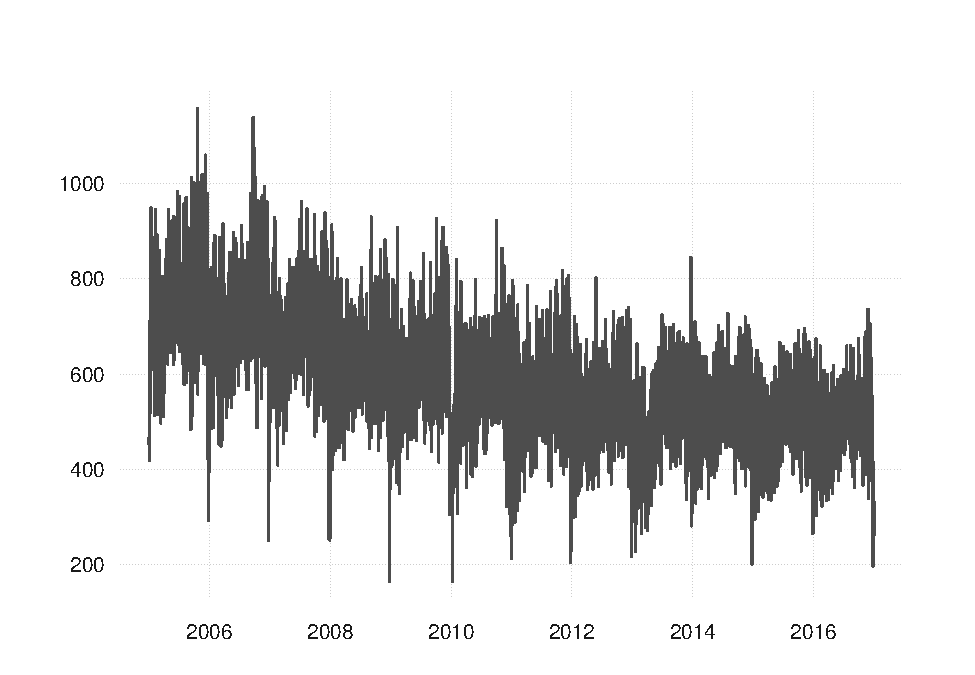
\includegraphics{overview_files/figure-latex/unnamed-chunk-1-1.pdf}

\hypertarget{arima-month-weekday-holiday-dummies}{%
\subsubsection{ARIMA + Month, Weekday / Holiday
Dummies}\label{arima-month-weekday-holiday-dummies}}

Let's start with a simple model.

Perhaps because of their simplicity, these kind of adjustments are
frequently found in the literature. E.g., timmermans 18, lengwiler,
(forthcoming, ask Ronald)

We start by constructing a dummy variables with weekday and monthly
effects:

\begin{Shaded}
\begin{Highlighting}[]
\NormalTok{dums <-}
\StringTok{  }\NormalTok{x }\OperatorTok
\StringTok{  }\KeywordTok{mutate}\NormalTok{(}\DataTypeTok{wday =}\NormalTok{ lubridate}\OperatorTok{::}\KeywordTok{wday}\NormalTok{(time, }\DataTypeTok{label =} \OtherTok{TRUE}\NormalTok{)) }\OperatorTok
\StringTok{  }\KeywordTok{mutate}\NormalTok{(}\DataTypeTok{month =}\NormalTok{ lubridate}\OperatorTok{::}\KeywordTok{month}\NormalTok{(time, }\DataTypeTok{label =} \OtherTok{TRUE}\NormalTok{)) }\OperatorTok
\StringTok{  }\KeywordTok{select}\NormalTok{(time, wday, month) }\OperatorTok
\StringTok{  }\NormalTok{fastDummies}\OperatorTok{::}\KeywordTok{dummy_cols}\NormalTok{(}\StringTok{"wday"}\NormalTok{, }\DataTypeTok{remove_selected_columns =} \OtherTok{TRUE}\NormalTok{) }\OperatorTok
\StringTok{  }\NormalTok{fastDummies}\OperatorTok{::}\KeywordTok{dummy_cols}\NormalTok{(}\StringTok{"month"}\NormalTok{, }\DataTypeTok{remove_selected_columns =} \OtherTok{TRUE}\NormalTok{) }\OperatorTok
\StringTok{  }\KeywordTok{select}\NormalTok{(}\OperatorTok{-}\NormalTok{wday_Mon, }\OperatorTok{-}\NormalTok{month_Jan)}

\NormalTok{dums}
\end{Highlighting}
\end{Shaded}

\begin{verbatim}
## # A tibble: 4,383 x 18
##    time       wday_Sun wday_Tue wday_Wed wday_Thu wday_Fri wday_Sat month_Feb
##    <date>        <int>    <int>    <int>    <int>    <int>    <int>     <int>
##  1 2005-01-01        0        0        0        0        0        1         0
##  2 2005-01-02        1        0        0        0        0        0         0
##  3 2005-01-03        0        0        0        0        0        0         0
##  4 2005-01-04        0        1        0        0        0        0         0
##  5 2005-01-05        0        0        1        0        0        0         0
##  6 2005-01-06        0        0        0        1        0        0         0
##  7 2005-01-07        0        0        0        0        1        0         0
##  8 2005-01-08        0        0        0        0        0        1         0
##  9 2005-01-09        1        0        0        0        0        0         0
## 10 2005-01-10        0        0        0        0        0        0         0
## # ... with 4,373 more rows, and 10 more variables: month_Mar <int>,
## #   month_Apr <int>, month_May <int>, month_Jun <int>, month_Jul <int>,
## #   month_Aug <int>, month_Sep <int>, month_Oct <int>, month_Nov <int>,
## #   month_Dec <int>
\end{verbatim}

These variables can be used as exogenous variables in a ARIMA model. We
use \texttt{forecat::auto.arima()} to determine the ARMA order. Note
that we do not want to use the seasonal part of the model, since we use
dummies for this purpose.

\begin{Shaded}
\begin{Highlighting}[]
\NormalTok{fit <-}\StringTok{ }\KeywordTok{auto.arima}\NormalTok{(x}\OperatorTok{$}\NormalTok{value, }\DataTypeTok{seasonal =} \OtherTok{FALSE}\NormalTok{, }\DataTypeTok{xreg =} \KeywordTok{as.matrix}\NormalTok{(dums[, }\DecValTok{-1}\NormalTok{]))}

\NormalTok{adj <-}\StringTok{ }\NormalTok{x}
\NormalTok{adj}\OperatorTok{$}\NormalTok{value <-}\StringTok{ }\KeywordTok{as.numeric}\NormalTok{(fit}\OperatorTok{$}\NormalTok{fitted)}

\KeywordTok{ts_plot}\NormalTok{(x, adj)}
\end{Highlighting}
\end{Shaded}

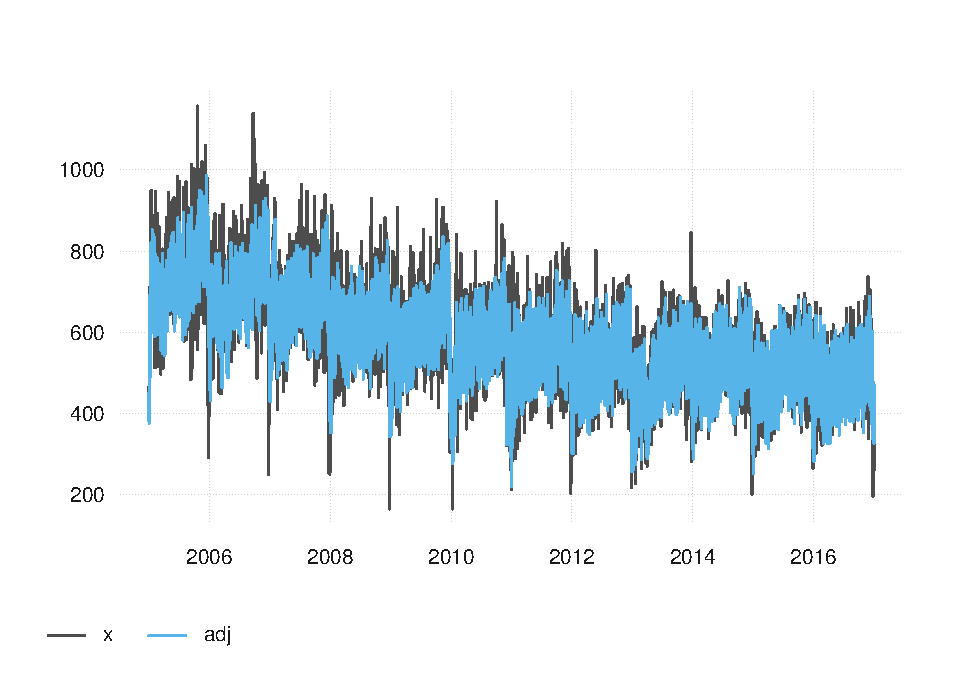
\includegraphics{overview_files/figure-latex/arimax-1.pdf}

The nice think about the dummy model is that its seasonal effects are
very easy to interprete. By construction, they are constant over time,
and can be visualized as follows:

\begin{Shaded}
\begin{Highlighting}[]
\KeywordTok{enframe}\NormalTok{(}\KeywordTok{coef}\NormalTok{(fit)) }\OperatorTok
\StringTok{  }\KeywordTok{filter}\NormalTok{(}\KeywordTok{grepl}\NormalTok{(}\StringTok{"wday"}\NormalTok{, name)) }\OperatorTok
\StringTok{  }\KeywordTok{mutate}\NormalTok{(}\DataTypeTok{name =} \KeywordTok{gsub}\NormalTok{(}\StringTok{"wday_"}\NormalTok{, }\StringTok{""}\NormalTok{, name)) }\OperatorTok
\StringTok{  }\KeywordTok{mutate}\NormalTok{(}\DataTypeTok{name =} \KeywordTok{factor}\NormalTok{(name, }\DataTypeTok{levels =} \KeywordTok{unique}\NormalTok{(name))) }\OperatorTok
\StringTok{  }\KeywordTok{ggplot}\NormalTok{(}\KeywordTok{aes}\NormalTok{(}\DataTypeTok{x =}\NormalTok{ name, }\DataTypeTok{y =}\NormalTok{ value)) }\OperatorTok{+}
\StringTok{    }\KeywordTok{geom_col}\NormalTok{() }\OperatorTok{+}
\StringTok{    }\KeywordTok{ggtitle}\NormalTok{(}\StringTok{"Weekday effects"}\NormalTok{, }\DataTypeTok{subtitle =} \StringTok{"Baseline: Monday"}\NormalTok{)}
\end{Highlighting}
\end{Shaded}

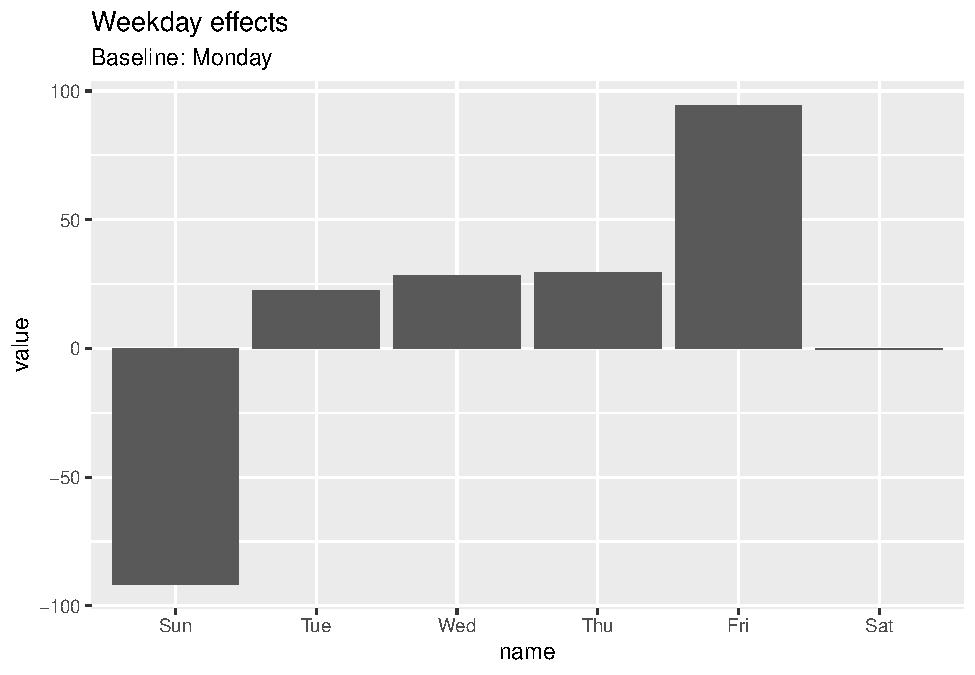
\includegraphics{overview_files/figure-latex/coeff-plots-1.pdf}

\begin{Shaded}
\begin{Highlighting}[]
\KeywordTok{enframe}\NormalTok{(}\KeywordTok{coef}\NormalTok{(fit)) }\OperatorTok
\StringTok{  }\KeywordTok{filter}\NormalTok{(}\KeywordTok{grepl}\NormalTok{(}\StringTok{"month"}\NormalTok{, name)) }\OperatorTok
\StringTok{  }\KeywordTok{mutate}\NormalTok{(}\DataTypeTok{name =} \KeywordTok{gsub}\NormalTok{(}\StringTok{"month_"}\NormalTok{, }\StringTok{""}\NormalTok{, name)) }\OperatorTok
\StringTok{  }\KeywordTok{mutate}\NormalTok{(}\DataTypeTok{name =} \KeywordTok{factor}\NormalTok{(name, }\DataTypeTok{levels =} \KeywordTok{unique}\NormalTok{(name))) }\OperatorTok
\StringTok{  }\KeywordTok{ggplot}\NormalTok{(}\KeywordTok{aes}\NormalTok{(}\DataTypeTok{x =}\NormalTok{ name, }\DataTypeTok{y =}\NormalTok{ value)) }\OperatorTok{+}
\StringTok{    }\KeywordTok{geom_col}\NormalTok{() }\OperatorTok{+}
\StringTok{    }\KeywordTok{ggtitle}\NormalTok{(}\StringTok{"Month effects"}\NormalTok{, }\DataTypeTok{subtitle =} \StringTok{"Baseline: January"}\NormalTok{)}
\end{Highlighting}
\end{Shaded}

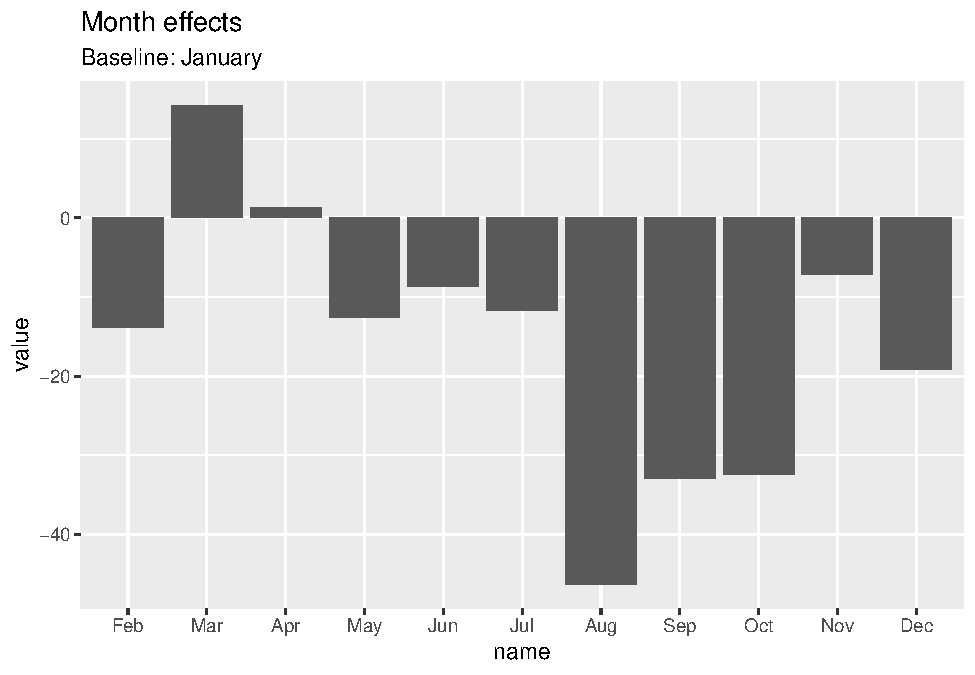
\includegraphics{overview_files/figure-latex/coeff-plots-2.pdf}

We see that, on average, transcations are lower on Sunday and peak on
Friday. We also see that, on average, transactions are sligthly lower in
early autumn.

\hypertarget{stl}{%
\subsubsection{STL}\label{stl}}

This package contains a very simple implementation of STL that works in
many circumstances.

\begin{Shaded}
\begin{Highlighting}[]
\KeywordTok{seas_daily}\NormalTok{(x) }\OperatorTok
\StringTok{  }\KeywordTok{ts_pick}\NormalTok{(}\StringTok{"orig"}\NormalTok{, }\StringTok{"adj"}\NormalTok{) }\OperatorTok
\StringTok{  }\KeywordTok{ts_plot}\NormalTok{()}
\end{Highlighting}
\end{Shaded}

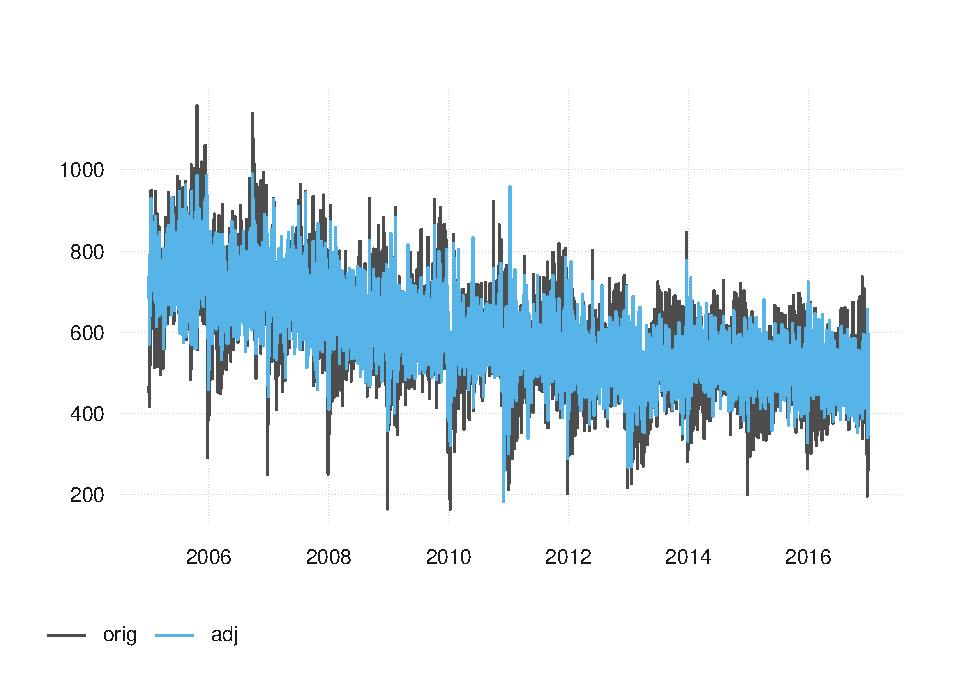
\includegraphics{overview_files/figure-latex/stl-1.pdf}

\hypertarget{dsa}{%
\subsubsection{dsa}\label{dsa}}

Similarly in spirit, the dsa packages implements a version of STL that
works well in many circumstances, but is computationally slow. The
following code automatlically decomposes \texttt{casulties}.

\begin{Shaded}
\begin{Highlighting}[]
\KeywordTok{library}\NormalTok{(dsa)}
\NormalTok{z <-}\StringTok{ }\NormalTok{dsa}\OperatorTok{::}\KeywordTok{dsa}\NormalTok{(}\KeywordTok{ts_xts}\NormalTok{(x))}
\end{Highlighting}
\end{Shaded}

\begin{verbatim}
##   |                                                                              |                                                                      |   0%  |                                                                              |===                                                                   |   5%  |                                                                              |=======                                                               |  10%  |                                                                              |====================                                                  |  29%  |                                                                              |===========================                                           |  38%  |                                                                              |===============================================                       |  67%  |                                                                              |==================================================                    |  71%  |                                                                              |=====================================================                 |  76%  |                                                                              |===============================================================       |  90%  |                                                                              |======================================================================| 100%
\end{verbatim}

\begin{Shaded}
\begin{Highlighting}[]
\KeywordTok{plot}\NormalTok{(z, }\DataTypeTok{dy =} \OtherTok{FALSE}\NormalTok{)}
\end{Highlighting}
\end{Shaded}

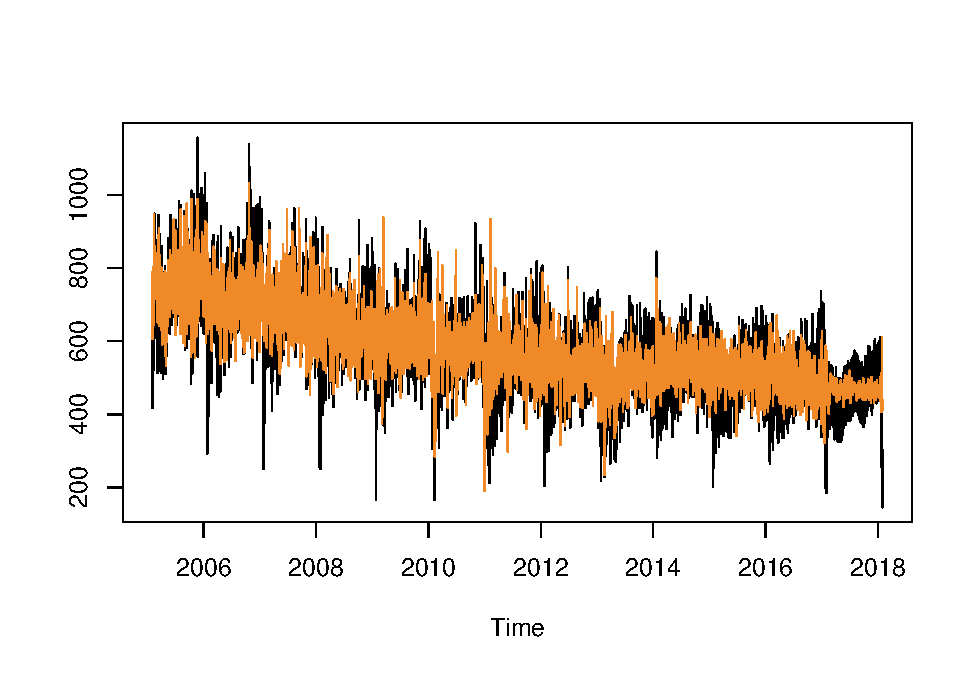
\includegraphics{overview_files/figure-latex/dsa-1.pdf}

\hypertarget{prophet}{%
\subsubsection{prophet}\label{prophet}}

\begin{Shaded}
\begin{Highlighting}[]
\KeywordTok{library}\NormalTok{(prophet)}
\end{Highlighting}
\end{Shaded}

\begin{verbatim}
## Loading required package: Rcpp
\end{verbatim}

\begin{verbatim}
## Loading required package: rlang
\end{verbatim}

\begin{verbatim}
## 
## Attaching package: 'rlang'
\end{verbatim}

\begin{verbatim}
## The following objects are masked from 'package:purrr':
## 
##     %@%, as_function, flatten, flatten_chr, flatten_dbl, flatten_int,
##     flatten_lgl, flatten_raw, invoke, list_along, modify, prepend,
##     splice
\end{verbatim}

\begin{Shaded}
\begin{Highlighting}[]
\NormalTok{df <-}\StringTok{ }\KeywordTok{rename}\NormalTok{(x, }\DataTypeTok{ds =}\NormalTok{ time, }\DataTypeTok{y =}\NormalTok{ value)}
\NormalTok{m <-}
\StringTok{  }\KeywordTok{prophet}\NormalTok{(}\DataTypeTok{daily.seasonality =} \OtherTok{FALSE}\NormalTok{) }\OperatorTok
\StringTok{  }\CommentTok{# including swiss holidays, which seems to have no effect}
\StringTok{  }\KeywordTok{add_country_holidays}\NormalTok{(}\DataTypeTok{country_name =} \StringTok{'CH'}\NormalTok{) }\OperatorTok
\StringTok{  }\KeywordTok{fit.prophet}\NormalTok{(df)}

\CommentTok{# not strictly needed, but will include forecast too}
\NormalTok{future <-}\StringTok{ }\KeywordTok{make_future_dataframe}\NormalTok{(m, }\DataTypeTok{periods =} \DecValTok{31}\NormalTok{)}
\NormalTok{forecast <-}\StringTok{ }\KeywordTok{as_tibble}\NormalTok{(}\KeywordTok{predict}\NormalTok{(m, future))}

\NormalTok{forecast }\OperatorTok
\StringTok{  }\KeywordTok{transmute}\NormalTok{(}
    \DataTypeTok{time =} \KeywordTok{as.Date}\NormalTok{(ds),}
\NormalTok{    additive_terms,}
\NormalTok{    yhat}
\NormalTok{  ) }\OperatorTok
\StringTok{  }\KeywordTok{left_join}\NormalTok{(x, }\DataTypeTok{by =} \StringTok{"time"}\NormalTok{) }\OperatorTok
\StringTok{  }\KeywordTok{mutate}\NormalTok{(}\DataTypeTok{adj =}\NormalTok{ value }\OperatorTok{-}\StringTok{ }\NormalTok{additive_terms) }\OperatorTok
\StringTok{  }\KeywordTok{select}\NormalTok{(time, value, adj) }\OperatorTok
\StringTok{  }\KeywordTok{ts_long}\NormalTok{() }\OperatorTok
\StringTok{  }\KeywordTok{ts_plot}\NormalTok{()}
\end{Highlighting}
\end{Shaded}

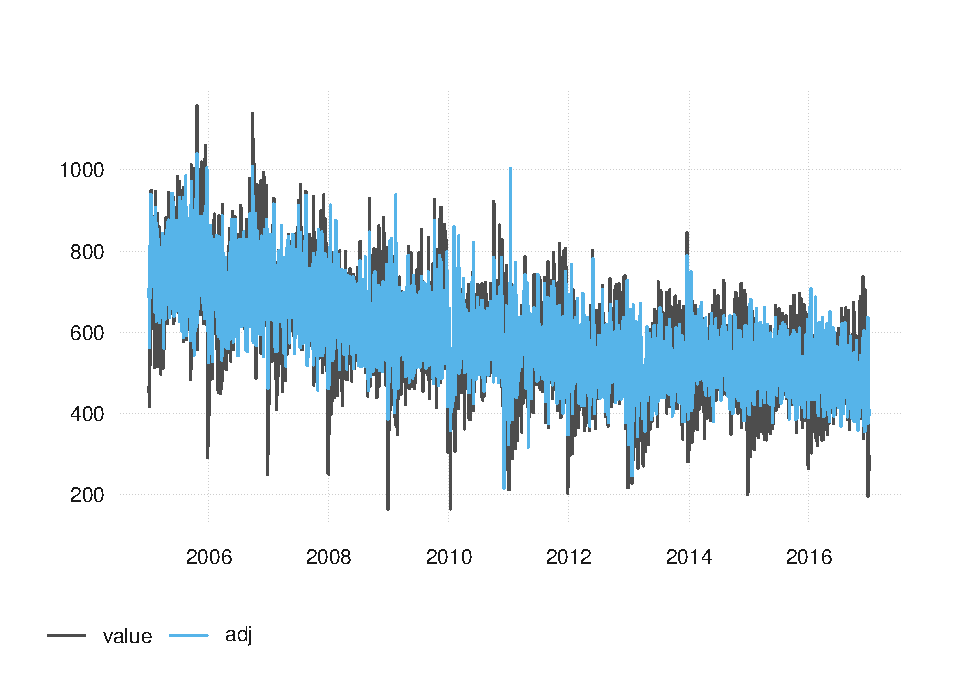
\includegraphics{overview_files/figure-latex/prophet-1.pdf}

\hypertarget{stlf}{%
\subsubsection{stlf}\label{stlf}}

Some models require the data to be equispaced. I.e., each low frequency
period must include the same number of high frequency periods.
\texttt{ts\_ts} from the tsbox package offers an easy way to convert
daily data into regular \texttt{"ts"} objects with a frequency of
365.2425. Thus, days are slightly offset in each year.

\begin{Shaded}
\begin{Highlighting}[]
\NormalTok{x_ts <-}\StringTok{ }\KeywordTok{ts_ts}\NormalTok{(x)}
\KeywordTok{head}\NormalTok{(x_ts)}
\end{Highlighting}
\end{Shaded}

\begin{verbatim}
## Time Series:
## Start = 2005 
## End = 2005.01368953503 
## Frequency = 365.2425 
## [1] 452 468 418 599 686 710
\end{verbatim}

{[}Probably don't show everything. This one is useless{]}

\begin{Shaded}
\begin{Highlighting}[]
\NormalTok{m <-}\StringTok{ }\KeywordTok{stlf}\NormalTok{(x_ts)}
\NormalTok{fct <-}\StringTok{ }\KeywordTok{ts_tbl}\NormalTok{(m}\OperatorTok{$}\NormalTok{mean)}
\NormalTok{adj <-}\StringTok{ }\NormalTok{m}\OperatorTok{$}\NormalTok{fitted}
\KeywordTok{ts_plot}\NormalTok{(x, adj)}
\end{Highlighting}
\end{Shaded}

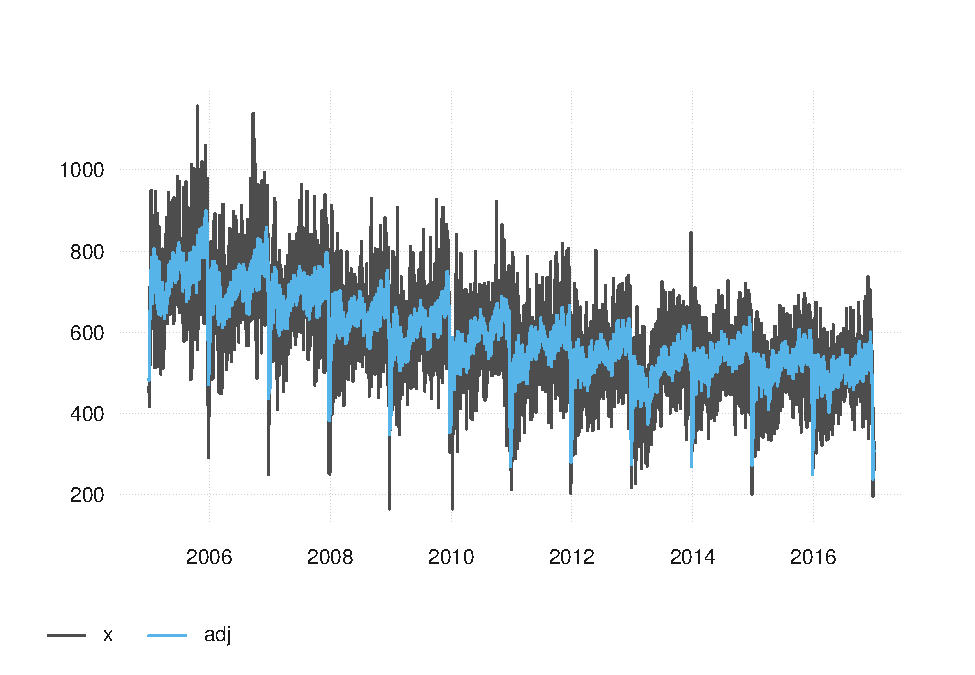
\includegraphics{overview_files/figure-latex/stlf-1.pdf}

\hypertarget{tbats}{%
\subsubsection{TBATS}\label{tbats}}

Other models require the data to be equispaced and without missing
values. Imputation offers an easy way out.

\begin{Shaded}
\begin{Highlighting}[]
\NormalTok{fit <-}\StringTok{ }\KeywordTok{tbats}\NormalTok{(imputeTS}\OperatorTok{::}\KeywordTok{na_interpolation}\NormalTok{(x_ts))}
\NormalTok{adj <-}\StringTok{ }\NormalTok{fit}\OperatorTok{$}\NormalTok{fitted}
\KeywordTok{ts_plot}\NormalTok{(x, adj)}
\end{Highlighting}
\end{Shaded}

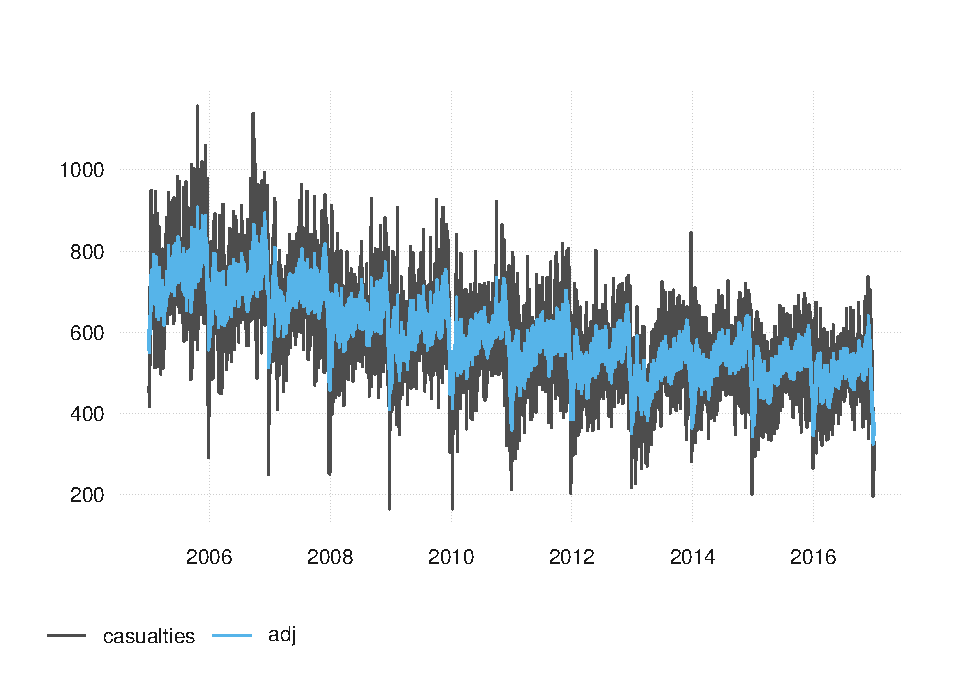
\includegraphics{overview_files/figure-latex/tbats-1.pdf}

\hypertarget{evaluation}{%
\subsection{Evaluation}\label{evaluation}}

Which method should you choose? {[}discuss criterions{]}

\hypertarget{out-of-sample-forecast}{%
\subsubsection{Out-of-sample forecast}\label{out-of-sample-forecast}}

As in (Timmermans 18), the following produces OOS forecasts for the
twelve last months for UK traffic deaths. We apply
\texttt{dailyseas::eval\_oos()} to perform an OOS forecast evaluation
for all models.

The full OOS results can be found
\href{https://github.com/christophsax/x13book/blob/master/topics/dailyadj/vignettes/overview.md}{here}

{[}I think the detailed OOS results are quite interesting, as they show
you what a method `gets' and what it does not.{]}

Here is the table for two series, showing the mean percentage deviation:

\begin{longtable}[]{@{}lrr@{}}
\toprule
model & casualties & transact\tabularnewline
\midrule
\endhead
dummy & 0.1564534 & 0.1554219\tabularnewline
daily & 0.1101139 & 0.1105550\tabularnewline
dsa & 0.0976475 & 0.1016794\tabularnewline
prophet & 0.1049195 & 0.1165156\tabularnewline
harmon & 0.1234707 & 0.1542884\tabularnewline
tbats & 0.1314058 & 0.1306881\tabularnewline
naive & 0.1402331 & 0.1710234\tabularnewline
\bottomrule
\end{longtable}

{[}The framework is now quite clean, so it is easy to include new
methods and series, or show other statistics{]}

prophet, dsa, and my stl work realatively good, the other methods are
not working very well.

\hypertarget{other-criteria}{%
\subsubsection{Other Criteria}\label{other-criteria}}

What other criteria could we look at?

\begin{itemize}
\item
  Variance?
\item
  Tests for remaining seasonality?
\item
  ???
\end{itemize}

\hypertarget{computation-time}{%
\subsubsection{Computation time}\label{computation-time}}

\begin{verbatim}
stl (my one): 0.639
seas_dummy:   2.319
prophet:     10.181
dsa:        145.553
\end{verbatim}

\hypertarget{other-challenges}{%
\subsection{Other challenges}\label{other-challenges}}

{[}Discuss some other challenges of daily seas adj{]}

\hypertarget{short-series}{%
\subsubsection{Short series}\label{short-series}}

Many daily time series are short. What does it mean with respect to the
discussion above. If I have only 3 years of data, which methods still
work?

\hypertarget{calendar-effects}{%
\subsubsection{Calendar effects}\label{calendar-effects}}

{[}Will try to improve my method on that, prophet and dsa do somehting
about it. Could provide an example, OOS comparison{]}

\hypertarget{cross-seasonal-effects}{%
\subsubsection{Cross Seasonal Effects}\label{cross-seasonal-effects}}

If month effects (e.g., salary payment at the end of a month) collide
with week effects (e.g., weekend), we can get some patterns that are
very hard to model. How relevant is the problem? What should you be done
about it?

\hypertarget{series-specific-effects}{%
\subsubsection{Series specific effects}\label{series-specific-effects}}

Transaction series have an end of months effect (Timmermans 18), but we
don't find it in other data. How to deal with such things?

\hypertarget{weekly-seasonality}{%
\subsubsection{Weekly seasonality}\label{weekly-seasonality}}

One solution would be to disaggregate, perform daily seasonal adjustment
and aggregate again. Could provide an example.

Compare to weekly methods?

\hypertarget{conclusions}{%
\subsection{Conclusions}\label{conclusions}}

\end{document}
